\subsection{Differensforstærker}
\label{Differensforstaerker}
%
Formålet med en differensforstærker er at forstærke spændingsforskellen mellem den inverterende og den ikke-inverterende terminal, uafhængigt af støj indfald. Da terminalerne er fysisk tæt på hinanden, så antages det at støj indfaldet er ens på begge terminaler, og derfor påvirker støjen ikke outputtet da differensforstærkeren undertrykker den uønskede støj. Evnen til at undertrykke støj kaldes \textit{Common Mode Rejection Ratio}, CMRR, desto større værdien er, desto bedre er differensforstærkeren til at undertrykke støj indfaldet. I forhold til kredsløbet sørger differensforstærkeren for, at spændingsforskellen mellem referencen og volumenkontrollen kun forstærkes én gang, hvorefter outputtet sendes uændret videre i kredsløbet. For at opnå én gangs forstærkning er det nødvendigt at alle modstandsværdierne i differensforstærkeren er ens, hvorfor de fire modstande alle har en modstand på 1M$\Omega$. At modstandende er på 1M$\Omega$ sørger for at indgangsimpedansen, set fra både volumenkontrollen og referencen, er meget stor. 
%
\begin{figure}[H]
	\centering
	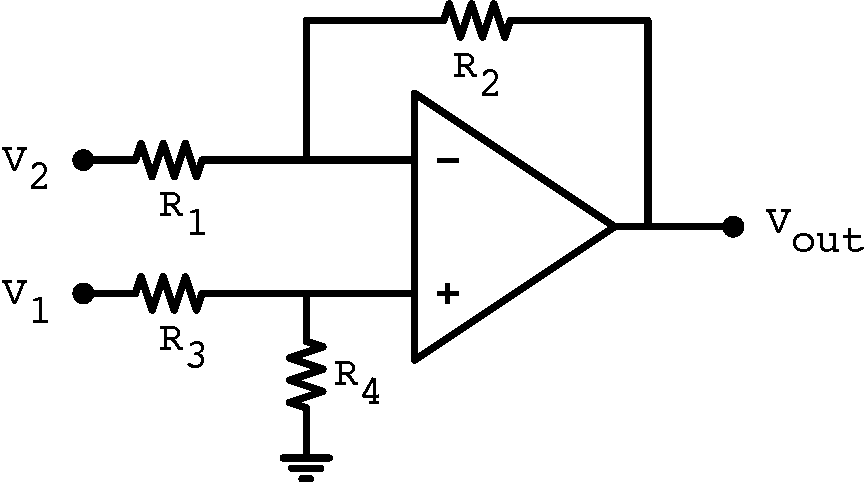
\includegraphics[resolution=300,scale=\circuitSize]{Figure/Circuits/Differensforstaerker.pdf}
	\caption{Kredsløbsdiagram for opkoblingen af en differensforstærker.}
	\label{fig:Differensforstaerker}
\end{figure}
\noindent
%
I \fullref{Differensforstaerker} illustreres opkoblingen af en differensforstærker, hvor $V_1$ er outputspændingen fra volumenkontrollen, som forbindes til den ikke-inverterende terminal og $V_2$ er outputspændingen fra referencen, som forbindes til den inverterende terminal. $V_{out}$ er spændingsforskellen mellem $V_1$ og $V_2$, som forbindes til en dobbeltensretter og en komparator.\\[5mm]
%
For at beregne outputtet fra differensforstærkeren anvendes superpositionsprincippet, hvor outputtet først regnes i forhold til $V_1$ hvor der ses bort fra $V_2$, og derefter omvendt. De to outputs skal normalvist adderes, men da differensforstærkeren har en inverterende tilbagekobling subtraheres de to outputs.\\[5mm]
%
For at beregne spændingen på den ikke-inverterende terminal, $V_+$, bruges udtrykket for spændingsdeling:
%
\begin{equation}
	V_+ = V_1*\left(\frac{R_4}{R_3+R_4}\right)
\end{equation}
%
\begin{equation}
	V_2 = 0
\end{equation}
%
For at beregne outputspændingen, $V_{out1}$, fra den ikke-inverterende terminal bruges følgende udtryk:
%
\begin{equation}
	V_{out1} = V_+*(G_+)= V_1*\left(\frac{R_4}{R_3+R_4}\right)*\left(\frac{R_1+R_2}{R_1}\right)
\end{equation}
%
For at beregne outputspændingen, $V_{out2}$, fra den inverterende terminal bruges følgende udtryk:
%
\begin{equation}
	V_{out2} = V_2*\left(-\frac{R_2}{R_1}\right)
\end{equation}
%
\begin{equation}
	V_1 = 0
\end{equation}
%
Da der bruges superpositionsprincippet skal outputspændingerne fra den inverterende og den ikke-inverterende terminal adderes med fortegn, da den inverterende terminal har et negativt fortegn, så subtraheres de to outputspændinger: 
%
\begin{equation}
	V_{out} = V_1*\left(\frac{R_4}{R_3+R_4}\right)*\left(\frac{R_1+R_2}{R_1}\right)-V_2*\left(\frac{R_2}{R_1}\right)
\end{equation}
% 
Da de fire modstande i differensforstærkeren er ens, 1M$\Omega$, så reduceres udtrykket til:
%
\begin{equation}
	V_{out} = V_1-V_2
\end{equation}
%
Så hvis $V_1$ > $V_2$ inderkerer det at volumenkontrollens outputspænding er større end referencens outputspænding, med andre ord er der skruet op for anlægget (>80dB), og derfor er outputtet fra differensforstærkeren positivt. Hvorimod hvis $V_1$ < $V_2$ så er volumenkontrollens outputspænding mindre end referencens outputspænding, med andre ord så er der blevet skruet ned for anlægget (<80dB) og derfor er outputtet fra differensforstærkeren negativt.\\[5mm] 
%
I kredsløbet er operationsforstærkeren brugt til differensforstærkeren én af de fire, der sidder i IC'en TL074, \parencite{PDF:OpAmp}. Differensforstærkeren er koblet til IC'ens anden operationsforstærker, hvor den ikke-inverterende terminal er på ben 5, den inverterende terminal er på ben 6 og outputtet er på ben 7, dertil forsynes IC'en med en $\pm 5V$ forsyningsspænding, på ben 4 $({V_{CC}}^+)$ og ben 11 $({V_{CC}}^-)$. 

IC'ens kan maksimalt forsynes med $\pm 18V$ og en maksimal inputspænding på de to terminaler på $\pm 15V$, hvilket hverken volumenkontrollen eller referencen opnår.

